\section{Results and Discussion}\label{sec:results}

All numbers in this section are test-set results of the single evaluation after freezing, reported as the mean $\pm$ standard deviation over \val{n-seeds} seeds; significance always refers to the seed-1 predictions with the Holm correction of Section~\ref{sec:stats}.

\subsection{Main comparison}\label{sec:main}

% Generated by paper/tools/make_tables.py. Do not edit by hand.
\begin{table*}[t]
\caption{Main comparison on the clean test sets: three-class Mendeley task and Super SMS (ham versus spam)}
\label{tab:main}
\centering\footnotesize\setlength{\tabcolsep}{3.5pt}
\begin{tabular}{lccccccc}
\hline
 & \multicolumn{6}{c}{Mendeley, three classes} & Super SMS \\
\cmidrule(lr){2-7}\cmidrule(lr){8-8}
Model & Macro F1 & Accuracy & F1 smishing & F1 spam & PR-AUC & ECE & Macro F1 \\
\hline
Cascade & 0.9316 $\pm$ 0.0074 & 0.9810 & 0.9181 & 0.8806 & 0.9445 & 0.0131 & 0.9934 $\pm$ 0.0005 \\ \hline
Char SVM, aug. (stage 1) & 0.9310 $\pm$ 0.0036 & 0.9803 & 0.9151 & 0.8825 & 0.9633 & 0.0184 & 0.9921 $\pm$ 0.0001 \\
Char SVM & \textbf{0.9374} $\pm$ 0.0000 & \textbf{0.9817} & \textbf{0.9239} & \textbf{0.8929} & \textbf{0.9659} & 0.0198 & 0.9925 $\pm$ 0.0000 \\
DistilBERT, aug. (stage 2) & 0.9149 $\pm$ 0.0115 & 0.9770 & 0.9069 & 0.8421 & 0.9617 & 0.0170 & 0.9932 $\pm$ 0.0007 \\
DistilBERT, stage-2 model, no aug. & 0.9183 $\pm$ 0.0108 & 0.9780 & 0.9081 & 0.8507 & 0.9554 & 0.0183 & -- \\
BERT & 0.9195 $\pm$ 0.0039 & 0.9779 & 0.9109 & 0.8519 & 0.9598 & 0.0179 & \textbf{0.9936} $\pm$ 0.0006 \\
TF-IDF + SVM & 0.9259 $\pm$ 0.0019 & 0.9791 & 0.9126 & 0.8697 & 0.9659 & 0.0187 & 0.9927 $\pm$ 0.0000 \\
TF-IDF + LR & 0.9181 $\pm$ 0.0012 & 0.9767 & 0.9239 & 0.8369 & 0.9616 & 0.0136 & 0.9909 $\pm$ 0.0000 \\
TF-IDF + RF & 0.9130 $\pm$ 0.0045 & 0.9732 & 0.8995 & 0.8488 & 0.9606 & 0.0875 & 0.9872 $\pm$ 0.0003 \\
TF-IDF + XGBoost & 0.8991 $\pm$ 0.0058 & 0.9667 & 0.8880 & 0.8233 & 0.9594 & \textbf{0.0110} & 0.9895 $\pm$ 0.0003 \\
TextCNN & 0.9006 $\pm$ 0.0129 & 0.9706 & 0.9085 & 0.8033 & 0.9424 & 0.0183 & 0.9891 $\pm$ 0.0002 \\
BiLSTM & 0.9104 $\pm$ 0.0106 & 0.9742 & 0.8925 & 0.8447 & 0.9413 & 0.0130 & 0.9897 $\pm$ 0.0005 \\
DistilBERT & 0.9103 $\pm$ 0.0113 & 0.9756 & 0.9023 & 0.8334 & 0.9509 & 0.0171 & 0.9929 $\pm$ 0.0003 \\
Qwen2.5-7B, few-shot & 0.8202 $\pm$ 0.0205 & 0.9455 & 0.7720 & 0.7029 & 0.8777 & 0.0407 & 0.8802 $\pm$ 0.0673 \\
\hline
\end{tabular}
\par\smallskip\footnotesize
Clean test sets; mean over 5 seeds ($\pm$ standard deviation for macro F1). Best value per column in bold (lowest for ECE). DistilBERT, stage-2 model: the second-stage architecture trained without augmentation; DistilBERT: the tuned baseline. For the few-shot model, class probabilities are the softmax over the logits of the first token of each label word. -- : not run in this condition.
\end{table*}


Table~\ref{tab:main} compares all models on the clean test sets. On the three-class Mendeley task, the highest macro F1 belongs to the character SVM without augmentation (\val{svmchar-clean-f1}). The cascade reaches \val{cascade-clean-f1}~$\pm$~\val{cascade-clean-f1-sd}, practically the same as its first stage alone (\val{svmcharaug-clean-f1}). On seed 1 the cascade is \val{clean-diff-abs} percentage points below the character SVM (95\% interval from \val{clean-ci-lo} to \val{clean-ci-hi}); the difference is not significant ($\tilde{p}=\val{clean-best-p-boot-holm}$ for the bootstrap and $\tilde{p}=\val{clean-best-p-mcn-holm}$ for the McNemar test). The fine-tuned transformers are lower on this task: BERT reaches \val{bert-clean-f1} and the second stage alone \val{distilaug-clean-f1}. The few-shot language model is the weakest model (\val{qwen-clean-f1}).

For all models the F1 score of the spam class is lower than that of the smishing class, and for the cascade most errors are confusions between these two malicious classes. For the cascade on seed 1 (Fig.~\ref{fig:confusion} in the Appendix), \val{cm-spam-to-smish} of the \val{men-test-spam} spam messages are labelled smishing and \val{cm-smish-to-spam} of the \val{men-test-smishing} smishing messages are labelled spam, while \val{cm-ham-wrong} of the \val{cm-ham-n} ham messages are misclassified. The cascade also has a lower calibration error (\val{ece-cascade}) than either of its stages (\val{ece-svmcharaug} and \val{ece-distilaug}). On the clean Super SMS corpus all trained models lie between \val{ss-min} and \val{ss-max}; the cascade (\val{ss-cascade}) and the best baseline, BERT (\val{ss-bert}), do not differ significantly ($\tilde{p}=\val{ss-p-boot}$ and $\val{ss-p-mcn}$).

\subsection{Settings of the published methods}\label{sec:published}

% Generated by paper/tools/make_tables.py. Do not edit by hand.
\begin{table*}[t]
\caption{Comparison with re-implemented published methods in their own task settings}
\label{tab:settings}
\centering\footnotesize\setlength{\tabcolsep}{3.5pt}
\begin{tabular}{lcccc}
\hline
Model & clean & HO 5\% & HO 10\% & HO 20\% \\
\hline
\multicolumn{5}{l}{\emph{Mahmud et al. setting: ham versus malicious}} \\
Cascade & 0.9877 $\pm$ 0.0027 & \textbf{0.9880} $\pm$ 0.0015 & 0.9873 $\pm$ 0.0013 & 0.9840 $\pm$ 0.0018 \\
Char SVM, aug. (stage 1) & 0.9836 $\pm$ 0.0007 & 0.9861 $\pm$ 0.0009 & 0.9833 $\pm$ 0.0018 & 0.9857 $\pm$ 0.0007 \\
Char SVM & 0.9864 $\pm$ 0.0009 & 0.9871 $\pm$ 0.0000 & \textbf{0.9886} $\pm$ 0.0000 & \textbf{0.9870} $\pm$ 0.0000 \\
DistilBERT, aug. (stage 2) & \textbf{0.9880} $\pm$ 0.0024 & 0.9880 $\pm$ 0.0015 & 0.9873 $\pm$ 0.0013 & 0.9840 $\pm$ 0.0018 \\
DistilBERT, stage-2 model, no aug. & 0.9866 $\pm$ 0.0013 & 0.9855 $\pm$ 0.0032 & 0.9703 $\pm$ 0.0112 & 0.9161 $\pm$ 0.0390 \\
BERT & 0.9838 $\pm$ 0.0030 & 0.9838 $\pm$ 0.0032 & 0.9793 $\pm$ 0.0045 & 0.9716 $\pm$ 0.0057 \\
TF-IDF + SVM & 0.9855 $\pm$ 0.0000 & 0.9838 $\pm$ 0.0000 & 0.9854 $\pm$ 0.0000 & 0.9704 $\pm$ 0.0000 \\
Mahmud et al., CNN-BiGRU & 0.9712 $\pm$ 0.0026 & 0.9497 $\pm$ 0.0048$^{\ast\ast\dagger\dagger}$ & 0.9205 $\pm$ 0.0079$^{\ast\ast\dagger\dagger}$ & 0.8555 $\pm$ 0.0084$^{\ast\ast\dagger\dagger}$ \\
\hline
\multicolumn{5}{l}{\emph{Shim et al. setting: smishing versus spam}} \\
Cascade & 0.9264 $\pm$ 0.0134 & 0.9220 $\pm$ 0.0114 & 0.9178 $\pm$ 0.0078 & 0.9080 $\pm$ 0.0098 \\
Char SVM, aug. (stage 1) & 0.9254 $\pm$ 0.0083 & 0.9188 $\pm$ 0.0072 & \textbf{0.9244} $\pm$ 0.0025 & 0.9222 $\pm$ 0.0046 \\
Char SVM & \textbf{0.9276} $\pm$ 0.0025 & \textbf{0.9232} $\pm$ 0.0000 & 0.9233 $\pm$ 0.0000 & \textbf{0.9233} $\pm$ 0.0000 \\
DistilBERT, aug. (stage 2) & 0.9089 $\pm$ 0.0148 & 0.9034 $\pm$ 0.0082 & 0.8676 $\pm$ 0.0169 & 0.8090 $\pm$ 0.0339 \\
DistilBERT, stage-2 model, no aug. & 0.8927 $\pm$ 0.0113 & 0.8946 $\pm$ 0.0173 & 0.8057 $\pm$ 0.0613 & 0.5519 $\pm$ 0.1202 \\
BERT & 0.9007 $\pm$ 0.0112 & 0.8992 $\pm$ 0.0279 & 0.7926 $\pm$ 0.0703 & 0.5755 $\pm$ 0.0976 \\
TF-IDF + SVM & 0.9196 $\pm$ 0.0031 & 0.9163 $\pm$ 0.0025 & 0.9232 $\pm$ 0.0000 & 0.9101 $\pm$ 0.0029 \\
Shim et al., BERT & 0.9027 $\pm$ 0.0186$^{\ast}$ & 0.8925 $\pm$ 0.0081$^{\ast\ast}$ & 0.7895 $\pm$ 0.0467$^{\ast\ast\dagger\dagger}$ & 0.5956 $\pm$ 0.0867$^{\ast\ast\dagger\dagger}$ \\
Shim et al., DistilBERT & 0.8935 $\pm$ 0.0174$^{\ast}$ & 0.8676 $\pm$ 0.0440 & 0.7109 $\pm$ 0.0751$^{\ast\ast\dagger\dagger}$ & 0.4416 $\pm$ 0.0663$^{\ast\ast\dagger\dagger}$ \\
Shim et al., RoBERTa & 0.8592 $\pm$ 0.0447$^{\ast\ast\dagger\dagger}$ & 0.8705 $\pm$ 0.0380$^{\ast\ast\dagger\dagger}$ & 0.8288 $\pm$ 0.0092$^{\ast\ast\dagger\dagger}$ & 0.6847 $\pm$ 0.1131$^{\ast\ast\dagger\dagger}$ \\
\hline
\end{tabular}
\par\smallskip\footnotesize
Macro F1, mean $\pm$ standard deviation over 5 seeds; best per column and setting in bold. HO: held-out obfuscation family at the given level. Marks on a published method (seed 1, Holm-adjusted, $\alpha=0.05$): $\ast$ the cascade is significantly better by one test (bootstrap or McNemar), $\ast\ast$ by both; $\dagger$ and $\dagger\dagger$ the same for the character SVM without augmentation (post-hoc comparison, not in the frozen plan). In every marked case the difference favours our model.
\end{table*}


The published papers report an accuracy of \val{claim-mh-acc} for the CNN-BiGRU of Mahmud et al. \cite{mahmud2024} and F1 scores between \val{claim-sh-min} and \val{claim-sh-max}\% for the BERT-family models of Shim et al. \cite{shim2024}. These values come from their own random splits without reported deduplication and with an unstated positive class, so they are not directly comparable with ours.

Table~\ref{tab:settings} shows the comparison in the task settings of these papers on our deduplicated data. On the clean test sets the differences between the cascade and the re-implemented methods are small. Against the CNN-BiGRU the difference is not significant; against the BERT and DistilBERT models of Shim et al. it is significant by the bootstrap test only, and against RoBERTa by both tests. Under held-out obfuscation the picture changes. The CNN-BiGRU falls to \val{mh-ho20} at the \val{lvl-c}\% level and the three models of Shim et al. to between \val{sh-ho20-min} and \val{sh-ho20-max}, while the cascade keeps \val{cascade-mahmud-ho20} and \val{cascade-shim-ho20}. These differences are significant by both tests at every held-out level in the Mahmud setting and at the \val{lvl-b}\% and \val{lvl-c}\% levels in the Shim setting; at \val{lvl-a}\% the difference to DistilBERT is not significant.

The post-hoc comparison (marks $\dagger$ in Table~\ref{tab:settings}) shows where this advantage comes from: the character SVM without augmentation is also significantly better than all re-implemented methods at the held-out levels where the cascade is, except at the \val{lvl-a}\% level of the Shim setting. On the clean test sets it is significantly better only than RoBERTa. The robustness of the cascade to obfuscation in these settings is therefore a property of its character-level first stage. In both settings the cascade does not differ significantly from our best baseline at any level (Table~\ref{tab:significance}).

% Generated by paper/tools/make_tables.py. Do not edit by hand.
\begin{table*}[t]
\caption{Cascade against the best baseline of each condition}
\label{tab:significance}
\centering\footnotesize\setlength{\tabcolsep}{2.5pt}
\begin{tabular}{lllccccccc}
\hline
Condition & Test & Best baseline & Cascade & Baseline & $\Delta$, pp & 95\% CI, pp & $b/c$ & $\tilde{p}$ boot. & $\tilde{p}$ McN. \\
\hline
Mendeley, 3 classes & clean & Char SVM & 0.9316 & 0.9374 & $-$1.85 & [$-$4.12, $+$0.32] & 2/7 & 0.088 & 0.180 \\
Mendeley, 3 classes & TR 5\% & Char SVM & 0.9237 & 0.9314 & $-$2.69 & [$-$5.39, $-$0.21] & 4/10 & \textbf{0.033} & 0.180 \\
Mendeley, 3 classes & TR 10\% & Char SVM & 0.9305 & 0.9343 & $-$0.96 & [$-$3.10, $+$1.10] & 3/6 & 0.362 & 0.508 \\
Mendeley, 3 classes & TR 20\% & Char SVM, aug. (stage 1) & 0.9210 & 0.9317 & $-$1.92 & [$-$4.38, $+$0.32] & 4/8 & 0.094 & 0.388 \\
Mendeley, 3 classes & HO 5\% & Char SVM, aug. (stage 1) & 0.9356 & 0.9338 & $-$0.70 & [$-$3.08, $+$1.58] & 6/6 & 0.561 & 1.000 \\
Mendeley, 3 classes & HO 10\% & Char SVM & 0.9384 & 0.9388 & $-$0.36 & [$-$1.92, $+$1.14] & 3/3 & 0.668 & 1.000 \\
Mendeley, 3 classes & HO 20\% & Char SVM, aug. (stage 1) & 0.9326 & 0.9336 & $-$0.22 & [$-$1.56, $+$1.04] & 2/2 & 0.730 & 1.000 \\
Low data 1\% & clean & Char SVM & 0.6957 & 0.7073 & $+$3.38 & [$-$0.56, $+$7.31] & 62/18 & 0.091 & \textbf{$<$0.001} \\
Low data 5\% & clean & Char SVM & 0.8145 & 0.8461 & $-$4.37 & [$-$8.62, $-$0.31] & 18/22 & \textbf{0.035} & 0.635 \\
Low data 10\% & clean & Char SVM & 0.8116 & 0.8843 & $-$9.38 & [$-$13.48, $-$5.48] & 9/29 & \textbf{$<$0.001} & \textbf{0.002} \\
Low data 25\% & clean & Char SVM & 0.8803 & 0.8996 & $-$1.63 & [$-$4.49, $+$1.17] & 8/12 & 0.258 & 0.503 \\
Mahmud setting & clean & DistilBERT, aug. (stage 2) & 0.9877 & 0.9880 & $+$0.00 & [$+$0.00, $+$0.00] & 0/0 & 1.000 & 1.000 \\
Mahmud setting & HO 5\% & DistilBERT, aug. (stage 2) & 0.9880 & 0.9880 & $+$0.00 & [$+$0.00, $+$0.00] & 0/0 & 1.000 & 1.000 \\
Mahmud setting & HO 10\% & Char SVM & 0.9873 & 0.9886 & $-$0.32 & [$-$1.22, $+$0.51] & 3/5 & 0.542 & 0.727 \\
Mahmud setting & HO 20\% & Char SVM & 0.9840 & 0.9870 & $-$0.48 & [$-$1.65, $+$0.64] & 5/8 & 0.427 & 0.581 \\
Shim setting & clean & Char SVM & 0.9264 & 0.9276 & $+$1.10 & [$-$1.09, $+$3.33] & 3/1 & 0.413 & 0.625 \\
Shim setting & HO 5\% & Char SVM & 0.9220 & 0.9232 & $+$1.65 & [$-$0.56, $+$4.37] & 4/1 & 0.361 & 0.578 \\
Shim setting & HO 10\% & Char SVM, aug. (stage 1) & 0.9178 & 0.9244 & $-$1.10 & [$-$4.34, $+$1.73] & 3/5 & 0.534 & 0.727 \\
Shim setting & HO 20\% & Char SVM & 0.9080 & 0.9233 & $-$2.19 & [$-$6.02, $+$1.62] & 4/8 & 0.263 & 0.388 \\
Transfer to MOZ & zero-shot & DistilBERT, aug. (stage 2) & 0.6115 & 0.6133 & $+$0.00 & [$+$0.00, $+$0.00] & 0/0 & 1.000 & 1.000 \\
Transfer to MOZ & fine-tuned & DistilBERT, aug. (stage 2) & 0.9705 & 0.9645 & $+$1.21 & [$+$0.28, $+$2.53] & 4/0 & \textbf{0.034} & 0.125 \\
Super SMS & clean & BERT & 0.9934 & 0.9936 & $-$0.08 & [$-$0.19, $+$0.04] & 19/28 & 0.214 & 0.243 \\
\hline
\end{tabular}
\par\smallskip\footnotesize
Cascade and baseline: mean macro F1 over 5 seeds. $\Delta$: macro F1 of the cascade minus that of the baseline on seed 1, in percentage points, with the 95\% paired bootstrap interval. $b/c$: test messages classified correctly only by the cascade / only by the baseline. $\tilde{p}$: Holm-adjusted $p$-values of the bootstrap and McNemar tests; values $\le 0.05$ in bold.
\end{table*}


\subsection{Robustness to obfuscation}\label{sec:robustness}

% Generated by paper/tools/make_tables.py. Do not edit by hand.
\begin{table*}[t]
\caption{Robustness to character obfuscation and ablations of the cascade}
\label{tab:robustness}
\centering\footnotesize\setlength{\tabcolsep}{2.5pt}
\begin{tabular}{lccccccc}
\hline
 & & \multicolumn{3}{c}{TRAIN family} & \multicolumn{3}{c}{HELD-OUT family} \\
\cmidrule(lr){3-5}\cmidrule(lr){6-8}
Model & clean & 5\% & 10\% & 20\% & 5\% & 10\% & 20\% \\
\hline
Cascade & 0.9316 $\pm$ 0.0074 & 0.9237 $\pm$ 0.0114 & 0.9305 $\pm$ 0.0062 & 0.9210 $\pm$ 0.0063 & 0.9356 $\pm$ 0.0068 & 0.9384 $\pm$ 0.0024 & 0.9326 $\pm$ 0.0046 \\
Char SVM, aug. (stage 1) & 0.9310 $\pm$ 0.0036 & 0.9290 $\pm$ 0.0062 & 0.9319 $\pm$ 0.0071 & \textbf{0.9317} $\pm$ 0.0024 & 0.9338 $\pm$ 0.0050 & 0.9329 $\pm$ 0.0069 & 0.9336 $\pm$ 0.0043 \\
Char SVM & \textbf{0.9374} $\pm$ 0.0000 & 0.9314 $\pm$ 0.0000 & \textbf{0.9343} $\pm$ 0.0017 & 0.9235 $\pm$ 0.0015 & 0.9317 $\pm$ 0.0011 & \textbf{0.9388} $\pm$ 0.0020 & 0.9322 $\pm$ 0.0019 \\
DistilBERT, aug. (stage 2) & 0.9149 $\pm$ 0.0115 & 0.9108 $\pm$ 0.0084 & 0.9011 $\pm$ 0.0069 & 0.8767 $\pm$ 0.0095 & 0.9202 $\pm$ 0.0084 & 0.9062 $\pm$ 0.0103 & 0.8872 $\pm$ 0.0101 \\
DistilBERT, stage-2 model, no aug. & 0.9183 $\pm$ 0.0108 & 0.9220 $\pm$ 0.0143 & 0.8510 $\pm$ 0.0186 & 0.6768 $\pm$ 0.0235 & 0.9262 $\pm$ 0.0085 & 0.8499 $\pm$ 0.0191 & 0.6462 $\pm$ 0.0284 \\
BERT & 0.9195 $\pm$ 0.0039 & 0.9166 $\pm$ 0.0073 & 0.8572 $\pm$ 0.0197 & 0.6999 $\pm$ 0.0631 & 0.9210 $\pm$ 0.0060 & 0.8625 $\pm$ 0.0194 & 0.6998 $\pm$ 0.0282 \\
TF-IDF + SVM & 0.9259 $\pm$ 0.0019 & 0.9180 $\pm$ 0.0024 & 0.9016 $\pm$ 0.0020 & 0.8894 $\pm$ 0.0043 & 0.9283 $\pm$ 0.0018 & 0.9259 $\pm$ 0.0023 & 0.9131 $\pm$ 0.0028 \\
TF-IDF + LR & 0.9181 $\pm$ 0.0012 & 0.9069 $\pm$ 0.0000 & 0.8813 $\pm$ 0.0000 & 0.8214 $\pm$ 0.0000 & 0.9107 $\pm$ 0.0000 & 0.8991 $\pm$ 0.0000 & 0.8716 $\pm$ 0.0000 \\
TF-IDF + RF & 0.9130 $\pm$ 0.0045 & 0.9237 $\pm$ 0.0039 & 0.8826 $\pm$ 0.0098 & 0.8213 $\pm$ 0.0137 & 0.9093 $\pm$ 0.0071 & 0.9004 $\pm$ 0.0067 & 0.8820 $\pm$ 0.0056 \\
TF-IDF + XGBoost & 0.8991 $\pm$ 0.0058 & 0.9016 $\pm$ 0.0088 & 0.8641 $\pm$ 0.0063 & 0.7865 $\pm$ 0.0089 & 0.9042 $\pm$ 0.0077 & 0.8797 $\pm$ 0.0084 & 0.8458 $\pm$ 0.0141 \\
TextCNN & 0.9006 $\pm$ 0.0129 & 0.8717 $\pm$ 0.0079 & 0.7896 $\pm$ 0.0225 & 0.6065 $\pm$ 0.0293 & 0.8651 $\pm$ 0.0062 & 0.7922 $\pm$ 0.0210 & 0.6249 $\pm$ 0.0313 \\
BiLSTM & 0.9104 $\pm$ 0.0106 & 0.8696 $\pm$ 0.0314 & 0.7945 $\pm$ 0.0507 & 0.6618 $\pm$ 0.0559 & 0.8623 $\pm$ 0.0380 & 0.7821 $\pm$ 0.0672 & 0.6073 $\pm$ 0.0861 \\
DistilBERT & 0.9103 $\pm$ 0.0113 & 0.9214 $\pm$ 0.0033 & 0.8344 $\pm$ 0.0253 & 0.6571 $\pm$ 0.0204 & 0.9321 $\pm$ 0.0061 & 0.8561 $\pm$ 0.0379 & 0.6790 $\pm$ 0.0538 \\
\hline
\multicolumn{8}{l}{\emph{Ablations of the cascade and earlier designs}} \\
Cascade without aug. & 0.9328 $\pm$ 0.0031 & \textbf{0.9347} $\pm$ 0.0034 & 0.9343 $\pm$ 0.0027 & 0.9222 $\pm$ 0.0037 & \textbf{0.9370} $\pm$ 0.0076 & 0.9322 $\pm$ 0.0051 & \textbf{0.9398} $\pm$ 0.0025 \\
Average of the two stages & 0.9297 $\pm$ 0.0085 & 0.9229 $\pm$ 0.0121 & 0.9163 $\pm$ 0.0095 & 0.9053 $\pm$ 0.0138 & 0.9326 $\pm$ 0.0085 & 0.9297 $\pm$ 0.0048 & 0.9241 $\pm$ 0.0064 \\
Gated fusion v1 & 0.9179 $\pm$ 0.0120 & 0.9149 $\pm$ 0.0105 & 0.8349 $\pm$ 0.0294 & 0.6654 $\pm$ 0.0482 & 0.9209 $\pm$ 0.0145 & 0.8178 $\pm$ 0.0312 & 0.6197 $\pm$ 0.0485 \\
Gated fusion v2, aug. & 0.9234 $\pm$ 0.0097 & 0.9240 $\pm$ 0.0025 & 0.9157 $\pm$ 0.0142 & 0.9156 $\pm$ 0.0138 & 0.9238 $\pm$ 0.0081 & 0.9252 $\pm$ 0.0084 & 0.9232 $\pm$ 0.0037 \\
Gated fusion v2 & 0.9189 $\pm$ 0.0161 & 0.9211 $\pm$ 0.0173 & 0.8797 $\pm$ 0.0186 & 0.7257 $\pm$ 0.0662 & 0.9253 $\pm$ 0.0148 & 0.8637 $\pm$ 0.0244 & 0.7027 $\pm$ 0.0875 \\
\hline
Cascade: share routed to stage 2, \% & 2.1 & 2.1 & 2.0 & 2.8 & 2.3 & 2.2 & 2.2 \\
\hline
\end{tabular}
\par\smallskip\footnotesize
Three-class Mendeley test set, macro F1, mean $\pm$ standard deviation over 5 seeds; best per column in bold. Percentages are obfuscation levels $\lambda$. The TRAIN family is used in the augmentation of the models marked aug.; the HELD-OUT family is never used in training.
\end{table*}


\begin{figure*}[t]
\centering
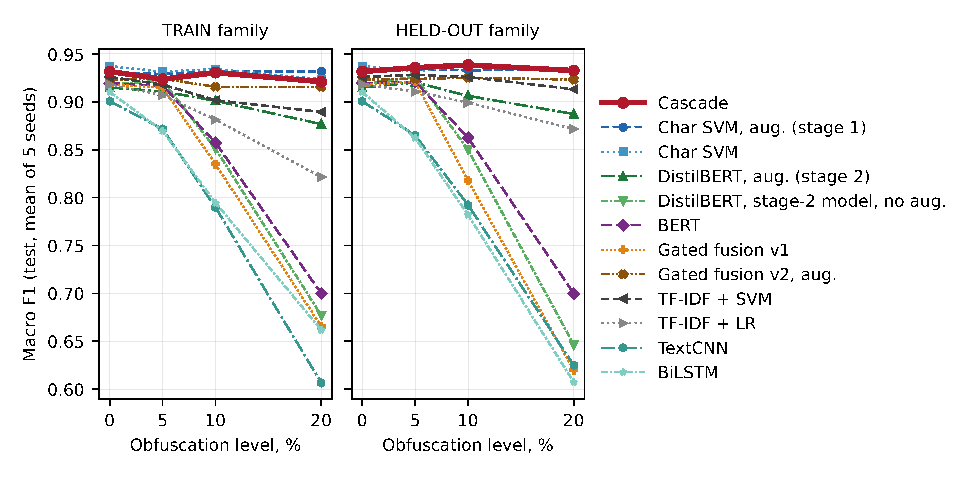
\includegraphics{figures/obfuscation_robustness}
\caption{Macro F1 on the three-class test set as a function of the obfuscation level, for the operation family used in augmentation (left) and the held-out family (right)}
\label{fig:obfuscation}
\end{figure*}

Table~\ref{tab:robustness} and Fig.~\ref{fig:obfuscation} show the three-class results under obfuscation. The realised share of edited characters matches the nominal level (for example \val{realised-ho20}\% at the \val{lvl-c}\% held-out level). Models that work on word or subword tokens without augmentation degrade strongly: at the \val{lvl-c}\% held-out level, BERT, the convolutional and recurrent networks, the tuned DistilBERT and the first gated fusion design reach only between \val{rob-neural-ho20-min} and \val{rob-neural-ho20-max}. Augmentation with the TRAIN family carries over to the unseen HELD-OUT family for the transformer: with the same architecture, the second stage reaches \val{rob-distilaug-ho20} with augmentation and \val{rob-distil-ho20} without it. The character-level models change little under either family: the character SVM without augmentation stays at \val{rob-svmchar-ho20}, and the cascade at \val{rob-cascade-ho20}. A plausible reason is that doubling a letter or deleting a vowel leaves most character n-grams of a message intact, and the sigmoid calibration keeps the confidence of the first stage high enough that the share routed to the second stage grows only slightly (from \val{routed-clean-pct}\% on the clean test set to at most \val{routed-max-pct}\%).

Against the best baseline of each obfuscated test set, the cascade is never significantly better (Table~\ref{tab:significance}); at the \val{lvl-a}\% TRAIN level it is significantly worse by the bootstrap test ($\tilde{p}=\val{tr05-p-boot}$), but not by the McNemar test.

\subsection{Low data and transfer}\label{sec:lowdata}

% Generated by paper/tools/make_tables.py. Do not edit by hand.
\begin{table*}[t]
\caption{Low-data regime and transfer to Portuguese messages}
\label{tab:lowdata}
\centering\footnotesize\setlength{\tabcolsep}{2.5pt}
\begin{tabular}{lccccccc}
\hline
 & \multicolumn{5}{c}{Share of the Mendeley training data} & \multicolumn{2}{c}{Transfer to MOZ-Smishing} \\
\cmidrule(lr){2-6}\cmidrule(lr){7-8}
Model & 1\% & 5\% & 10\% & 25\% & 100\% & zero-shot & fine-tuned \\
\hline
Cascade & 0.6957 $\pm$ 0.0312 & 0.8145 $\pm$ 0.0177 & 0.8116 $\pm$ 0.0146 & 0.8803 $\pm$ 0.0170 & 0.9316 $\pm$ 0.0074 & 0.6115 $\pm$ 0.0174 & \textbf{0.9705} $\pm$ 0.0037 \\
Char SVM, aug. (stage 1) & 0.6972 $\pm$ 0.0115 & 0.8370 $\pm$ 0.0095 & 0.8685 $\pm$ 0.0086 & 0.8917 $\pm$ 0.0077 & 0.9310 $\pm$ 0.0036 & 0.5091 $\pm$ 0.0122 & 0.9320 $\pm$ 0.0058 \\
Char SVM & \textbf{0.7073} $\pm$ 0.0100 & \textbf{0.8461} $\pm$ 0.0041 & \textbf{0.8843} $\pm$ 0.0026 & \textbf{0.8996} $\pm$ 0.0021 & \textbf{0.9374} $\pm$ 0.0000 & 0.5184 $\pm$ 0.0020 & 0.9423 $\pm$ 0.0047 \\
DistilBERT, aug. (stage 2) & 0.5418 $\pm$ 0.1481 & 0.7276 $\pm$ 0.0508 & 0.7366 $\pm$ 0.0586 & 0.8529 $\pm$ 0.0187 & 0.9149 $\pm$ 0.0115 & \textbf{0.6133} $\pm$ 0.0193 & 0.9645 $\pm$ 0.0039 \\
DistilBERT, stage-2 model, no aug. & 0.5988 $\pm$ 0.0697 & 0.7823 $\pm$ 0.0503 & 0.8036 $\pm$ 0.0185 & 0.8564 $\pm$ 0.0201 & 0.9183 $\pm$ 0.0108 & 0.5773 $\pm$ 0.0456 & 0.9617 $\pm$ 0.0049 \\
BERT & 0.3341 $\pm$ 0.0663 & 0.5960 $\pm$ 0.0772 & 0.7865 $\pm$ 0.0411 & 0.8362 $\pm$ 0.0307 & 0.9195 $\pm$ 0.0039 & -- & -- \\
TF-IDF + SVM & 0.6651 $\pm$ 0.0175 & 0.8036 $\pm$ 0.0108 & 0.8575 $\pm$ 0.0055 & 0.8762 $\pm$ 0.0023 & 0.9259 $\pm$ 0.0019 & 0.3859 $\pm$ 0.0016 & 0.9601 $\pm$ 0.0000 \\
TF-IDF + LR & 0.6363 $\pm$ 0.0000 & 0.7171 $\pm$ 0.0000 & 0.8519 $\pm$ 0.0000 & 0.8669 $\pm$ 0.0000 & 0.9181 $\pm$ 0.0012 & 0.4162 $\pm$ 0.0000 & 0.9571 $\pm$ 0.0000 \\
Gated fusion v1 & 0.6247 $\pm$ 0.0684 & 0.7736 $\pm$ 0.0105 & 0.8118 $\pm$ 0.0153 & 0.8518 $\pm$ 0.0131 & 0.9179 $\pm$ 0.0120 & 0.5536 $\pm$ 0.0254 & 0.9635 $\pm$ 0.0081 \\
Gated fusion v2, aug. & 0.3640 $\pm$ 0.1330 & 0.7814 $\pm$ 0.0616 & 0.7641 $\pm$ 0.0389 & 0.8663 $\pm$ 0.0097 & 0.9234 $\pm$ 0.0097 & -- & -- \\
\hline
Cascade: share routed to stage 2, \% & 17.9 & 9.2 & 7.8 & 5.3 & 2.1 & 68.4 & 77.3 \\
\hline
\end{tabular}
\par\smallskip\footnotesize
Macro F1 on the clean test set, mean $\pm$ standard deviation over 5 seeds; best per column in bold. Low data: three-class Mendeley task, nested stratified subsets of the training data, cascade with the frozen $\tau^{*}$. Transfer: trained on ham versus malicious in the Mendeley corpus, tested on MOZ-Smishing without target data (zero-shot) and after fine-tuning on 10\% of its training data; the transformer is the multilingual DistilBERT. -- : not run in this condition.
\end{table*}


\begin{figure*}[t]
\centering
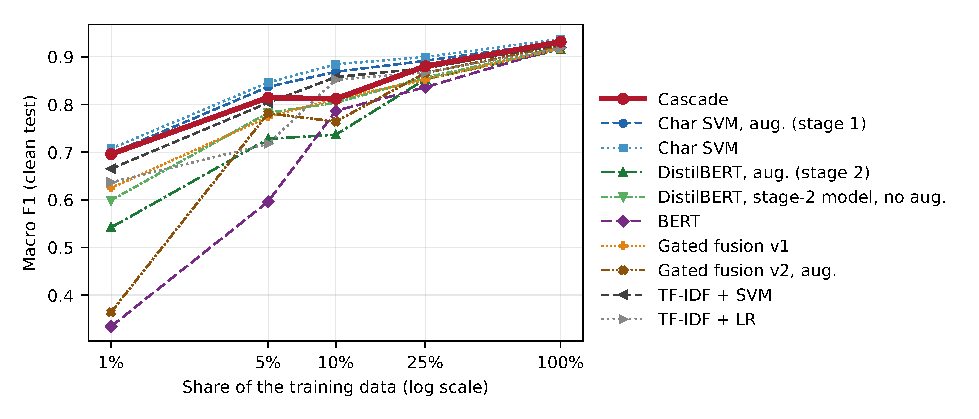
\includegraphics{figures/learning_curve}
\caption{Macro F1 on the clean three-class test set as a function of the share of the training data}
\label{fig:learning}
\end{figure*}

With less training data (Table~\ref{tab:lowdata}, Fig.~\ref{fig:learning}) the character SVM without augmentation has the highest mean macro F1 among the baselines at every fraction, and the cascade falls behind it. (The average of the two stages, an ablation, is higher at \val{ld-a}\% and \val{ld-b}\%, with \val{ld01-average} and \val{ld05-average}.) With \val{ld-c}\% of the data the cascade reaches \val{ld10-cascade} against \val{ld10-svmchar}, a significant difference by both tests; at \val{ld-b}\% the difference is significant by the bootstrap test only. At \val{ld-a}\% the McNemar test on seed 1 favours the cascade (\val{ld01-b} messages correct only for the cascade against \val{ld01-c}), but the bootstrap test is not significant and the mean over seeds is lower (\val{ld01-cascade} against \val{ld01-svmchar}). The reason is visible in the last row of the table: the frozen threshold sends \val{ld01-share}\% of the messages to the second stage at \val{ld-a}\% of the data, and the transformer trained on so few messages is weak (\val{ld01-distilaug}).

Transfer from English to Portuguese without target data fails for all models: the best mean macro F1 is \val{tr-zs-best}. With the threshold chosen on the source validation data ($\tau=\val{tau-tr-zs}$), the cascade sends \val{tr-zs-share}\% of the messages to the second stage and is identical to it on seed 1. After fine-tuning on \val{tr-frac}\% of the target training data, the cascade reaches \val{tr-ft-cascade} against \val{tr-ft-distilaug} for its second stage alone, a difference that is significant by the bootstrap test only ($\tilde{p}=\val{tr-ft-p-boot}$); the average of the two stages has the highest mean (\val{tr-ft-average}) but was not tested. In this condition, too, most messages reach the transformer (\val{tr-ft-share}\%), so the cascade offers no saving in computation.

\subsection{Cost of errors}\label{sec:costres}

The cost columns of Table~\ref{tab:efficiency} give $L_r$ in the ham-versus-malicious view. On the clean test set the lowest loss for every $r$ belongs to the average of the two stages, an ablation (\val{cost-clean-r3-average} for $r=\val{cost-r3}$). Among the other models the cascade has the lowest loss for $r=\val{cost-r1}$ (\val{cost-clean-r1-cascade}), and the second stage alone for $r=\val{cost-r2}$ and $r=\val{cost-r3}$, with the cascade close to it (\val{cost-clean-r3-cascade} against \val{cost-clean-r3-distilaug} for $r=\val{cost-r3}$). At the \val{lvl-c}\% held-out level the cascade has the lowest loss of all models for every $r$; for $r=\val{cost-r2}$ it is \val{cost-ho20-r2-cascade} against \val{cost-ho20-r2-svmcharaug} for its first stage and \val{cost-ho20-r2-distilaug} for its second stage. The cascade is not the cheapest everywhere: in the Mahmud setting at the same level its loss for $r=\val{cost-r2}$ is \val{cost-mh-ho20-r2-cascade} against \val{cost-mh-ho20-r2-svmcharaug} for the character SVM with augmentation, because there it mostly answers with the transformer. Differences in $L_r$ were not tested for significance.

\subsection{Speed and the quality-latency trade-off}\label{sec:speed}

% Generated by paper/tools/make_tables.py. Do not edit by hand.
\begin{table*}[t]
\caption{Efficiency and cost of errors on the three-class task}
\label{tab:efficiency}
\centering\footnotesize\setlength{\tabcolsep}{2.5pt}
\begin{tabular}{lcccccccccc}
\hline
 & \multicolumn{4}{c}{CPU, one thread, batch 1} & \multicolumn{3}{c}{$L_r$, clean} & \multicolumn{3}{c}{$L_r$, HO 20\%} \\
\cmidrule(lr){2-5}\cmidrule(lr){6-8}\cmidrule(lr){9-11}
Model & p50, ms & p95, ms & msg/s & MB & $r=1$ & $r=5$ & $r=10$ & $r=1$ & $r=5$ & $r=10$ \\
\hline
TextCNN & 0.95 & 1.17 & 1059 & 6.1 & 0.0169 & 0.0789 & 0.1564 & 0.0659 & 0.3167 & 0.6303 \\
TF-IDF + XGBoost & 1.07 & 1.41 & 892 & 1.3 & 0.0235 & 0.0981 & 0.1913 & 0.0404 & 0.2021 & 0.4042 \\
Char SVM, aug. (stage 1) & 1.46 & 1.73 & 669 & 6.6 & 0.0077 & 0.0251 & 0.0469 & 0.0080 & 0.0303 & 0.0582 \\
Char SVM & 1.47 & 1.87 & 660 & 5.4 & 0.0078 & 0.0253 & 0.0470 & 0.0080 & 0.0331 & 0.0645 \\
Cascade & 1.60 & 2.47 & 297 & 272.9 & \textbf{0.0064} & 0.0204 & 0.0378 & \textbf{0.0064} & \textbf{0.0260} & \textbf{0.0503} \\
TF-IDF + LR & 1.67 & 2.07 & 582 & 3.2 & 0.0111 & 0.0523 & 0.1037 & 0.0340 & 0.1664 & 0.3319 \\
TF-IDF + SVM & 2.49 & 3.12 & 391 & 2.3 & 0.0077 & 0.0237 & 0.0437 & 0.0209 & 0.0920 & 0.1808 \\
BiLSTM & 2.65 & 5.91 & 316 & 7.6 & 0.0103 & 0.0312 & 0.0573 & 0.0584 & 0.2340 & 0.4535 \\
DistilBERT, stage-2 model, no aug. & 41.72 & 76.27 & 21 & 266.3 & 0.0066 & 0.0226 & 0.0427 & 0.0469 & 0.2308 & 0.4608 \\
DistilBERT, aug. (stage 2) & 41.84 & 76.01 & 21 & 266.3 & 0.0070 & \textbf{0.0202} & \textbf{0.0368} & 0.0099 & 0.0364 & 0.0695 \\
Gated fusion v1 & 42.14 & 76.46 & 21 & 267.4 & 0.0075 & 0.0249 & 0.0467 & 0.0422 & 0.2073 & 0.4138 \\
DistilBERT & 42.79 & 81.63 & 20 & 268.5 & 0.0078 & 0.0239 & 0.0439 & 0.0376 & 0.1798 & 0.3575 \\
TF-IDF + RF & 44.30 & 47.27 & 22 & 27.7 & 0.0160 & 0.0753 & 0.1493 & 0.0350 & 0.1751 & 0.3502 \\
Gated fusion v2, aug. & 76.48 & 111.80 & 12 & 409.4 & 0.0066 & 0.0213 & 0.0395 & 0.0084 & 0.0341 & 0.0664 \\
Gated fusion v2 & 77.33 & 114.47 & 12 & 409.4 & 0.0066 & 0.0213 & 0.0395 & 0.0432 & 0.2118 & 0.4226 \\
BERT & 84.67 & 159.07 & 10 & 438.7 & 0.0073 & 0.0206 & 0.0371 & 0.0347 & 0.1699 & 0.3389 \\
Qwen2.5-7B, few-shot$^{a}$ & 178.10 & -- & -- & 5443.3 & 0.0240 & 0.0505 & 0.0836 & -- & -- & -- \\
\hline
\end{tabular}
\par\smallskip\footnotesize
Latency per message on the three-class Mendeley test messages; the cascade is measured end to end on the whole test set, including the calls of the second stage. Size: saved model files. $L_r$: loss per message (\ref{eq:cost}) in the ham-versus-malicious view, mean over 5 seeds; lowest per column in bold. $^{a}$ 4-bit model on a T4 GPU (median only), not comparable with the CPU rows.
\end{table*}


\begin{figure*}[t]
\centering
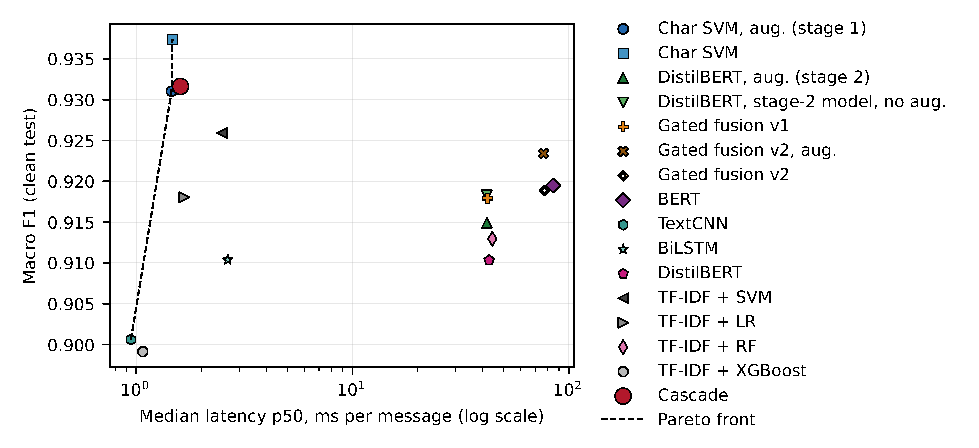
\includegraphics{figures/quality_vs_latency}
\caption{Macro F1 on the clean three-class test set against the median latency per message on one CPU thread; the dashed line is the Pareto front}
\label{fig:pareto}
\end{figure*}

Measured end to end on all \val{men-test-n} test messages, the cascade has a median latency of \val{lat-cascade-p50}~ms, a 95th percentile of \val{lat-cascade-p95}~ms and a throughput of \val{lat-cascade-thr} messages per second on one CPU thread, with \val{lat-cascade-routed-pct}\% of the messages sent to the second stage (Table~\ref{tab:efficiency}). Its mean latency, \val{lat-cascade-mean}~ms, is about twice the median, because each routed message costs a full transformer call. For comparison, the first stage alone has a median of \val{lat-svmcharaug-p50}~ms (\val{lat-svmcharaug-thr} messages per second), DistilBERT \val{lat-distilaug-p50}~ms and BERT \val{lat-bert-p50}~ms. The few-shot language model needs \val{lat-qwen-p50}~ms per message even on a GPU.

Fig.~\ref{fig:pareto} places these results on the quality-latency plane. The character SVM without augmentation is on the Pareto front; the cascade lies slightly below it in clean macro F1 and needs more time and memory, mainly the \val{size-cascade} MB of the transformer weights. On clean data, therefore, the cascade buys nothing over its first stage. What it adds is the fallback to a transformer for low-confidence messages, at a mean cost per message that stays within a few milliseconds, and the lowest error cost under strong obfuscation.

\subsection{Analysis}\label{sec:analysis}

\begin{figure}[t]
\centering
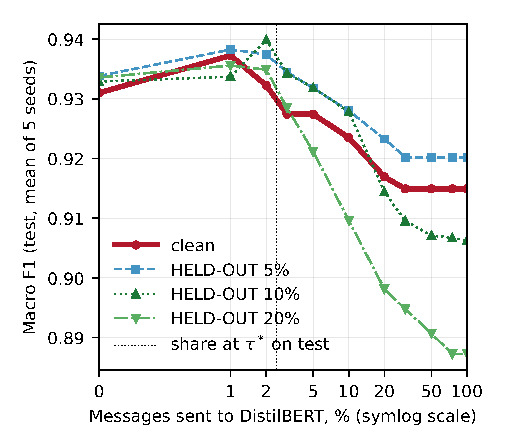
\includegraphics{figures/cascade_share_vs_f1}
\caption{Macro F1 of the cascade when a given share of the test messages with the lowest first-stage confidence is sent to the second stage (descriptive, not used for any choice). HO: held-out obfuscation family; dotted line: share sent at the frozen threshold}
\label{fig:share}
\end{figure}

\emph{What the second stage contributes.} Fig.~\ref{fig:share} varies the share of test messages sent to the second stage, always choosing those with the lowest first-stage confidence. On the clean test set the macro F1 rises from \val{curve-clean-0} with no routing to \val{curve-clean-peak} at \val{curve-clean-peak-share}\% and then falls to \val{curve-clean-100} when every message goes to the transformer; the held-out sets behave similarly. A small share of uncertain messages thus benefits from the transformer, and the frozen threshold, with \val{lat-cascade-routed-pct}\% on the test set, lies in this region. The curve is computed on the test set and is descriptive only.

\emph{Ablations.} The cascade of the two models trained without augmentation (Table~\ref{tab:robustness}) has a higher mean macro F1 than the final cascade on \val{noaug-wins} of the \val{n-rob-sets} three-class test sets, all except the \val{lvl-b}\% held-out set; only \val{noaug-beyond} of these differences exceeds the seed spread. Augmentation therefore did not improve the cascade on test, although it is essential for the transformer alone. Averaging the probabilities of the two stages is lower than the cascade under every obfuscation level.

\emph{Earlier designs.} The two gated fusion models of a DistilBERT representation with hand-crafted features are not better than the character SVM on any test set. The first design degrades under obfuscation like the other transformers (\val{rob-v1-ho20} at the \val{lvl-c}\% held-out level); the second, with character features and augmentation, is robust (\val{rob-v2-ho20}) but lower and about \val{v2-slowdown} times slower than the cascade. We report them as negative results; they were developed on validation data before the final design was frozen.

\emph{Label noise between smishing and spam.} The boundary between the two malicious classes is not labelled consistently in the Mendeley corpus. All \val{men-conflict-groups} groups of duplicates with conflicting labels pair a smishing and a spam label on the same or nearly the same text, and of the \val{men-uci-smish} deduplicated Mendeley smishing messages, \val{men-smish-uci-spam} have a duplicate in the UCI collection, where they are labelled spam. Part of the remaining confusion between these classes is therefore likely to come from the labels rather than from the models.

% Generated by paper/tools/make_tables.py. Do not edit by hand.
\begin{table*}[t]
\caption{Effect of duplicates on cross-validated scores (dirty minus clean data)}
\label{tab:inflation}
\centering\footnotesize\setlength{\tabcolsep}{2.5pt}
\begin{tabular}{lllccccccc}
\hline
 & & & \multicolumn{3}{c}{Accuracy} & \multicolumn{3}{c}{Macro F1} & \\
\cmidrule(lr){4-6}\cmidrule(lr){7-9}
Model & Task & $n$ dirty/clean & dirty & clean & $\Delta$, pp & dirty & clean & $\Delta$, pp & dup., \% \\
\hline
TF-IDF + SVM & 3 classes & 4801/4591 & 0.9582 & 0.9714 & $-$1.32 & 0.8637 & 0.8993 & $-$3.57 & 5.5 \\
TF-IDF + LR & 3 classes & 4801/4591 & 0.9551 & 0.9686 & $-$1.35 & 0.8551 & 0.8912 & $-$3.61 & 5.5 \\
Mahmud et al., CNN-BiGRU & ham vs mal. & 4801/4591 & 0.9824 & 0.9800 & $+$0.24 & 0.9710 & 0.9613 & $+$0.96 & 5.5 \\
Shim et al., BERT & smish. vs spam & 923/731 & 0.8411 & 0.8768 & $-$3.58 & 0.8377 & 0.8748 & $-$3.72 & 25.4 \\
Shim et al., DistilBERT & smish. vs spam & 923/731 & 0.8360 & 0.8892 & $-$5.31 & 0.8306 & 0.8883 & $-$5.77 & 25.4 \\
Shim et al., RoBERTa & smish. vs spam & 923/731 & 0.7161 & 0.7457 & $-$2.96$^{a}$ & 0.6147 & 0.6791 & $-$6.43$^{a}$ & 25.4 \\
\hline
\end{tabular}
\par\smallskip\footnotesize
Five-fold cross-validation on the training and validation parts of the Mendeley corpus; mean over 3 seeds. Dirty: all raw messages except those whose duplicate group is kept in our test part, with the raw labels; clean: our deduplicated data. dup.: share of dirty test-fold messages with a duplicate in the training folds. $^{a}$ difference within the larger seed standard deviation.
\end{table*}


\emph{Duplicates and inflated scores.} Table~\ref{tab:inflation} compares five-fold cross-validation on the raw Mendeley data with the same procedure on our deduplicated data. In the binary ham-versus-malicious task, the raw data give higher scores: for the CNN-BiGRU, accuracy is higher by \val{infl-mh-acc} and macro F1 by \val{infl-mh-f1} percentage points, and the raw-data accuracy (\val{infl-mh-acc-dirty}) is close to the value reported in the original paper (\val{claim-mh-acc}). In the three-class and smishing-versus-spam tasks the raw data give \emph{lower} scores, by up to \val{infl-max-drop} points of macro F1. The raw data keep both members of the conflicting smishing and spam pairs, which give contradictory training and test labels; in the binary task both labels are malicious and the conflict disappears. The analysis therefore mixes two effects, duplicates and conflicting labels, which we did not separate. It shows that the treatment of duplicates changes the scores by several points in either direction, which is larger than most differences between models in Table~\ref{tab:main}.

\subsection{Case study: Kazakhstan}\label{sec:kz}

The models above were trained on English messages. To see how they behave in a different context, we wrote a small set of messages for Kazakhstan, where text messages are commonly written in Russian or Kazakh. This part is a qualitative demonstration with a few dozen messages, not a statistical evaluation, and the translation and adaptation experiments were added after the main results (post hoc).

\emph{Messages.} Seven scenarios (a bank card blocked, a prize, an expiring digital signature, a parcel held for payment, early pension withdrawal, a bonus for a code, a call from a bank security service) each have a fraudulent message and a legitimate counterpart, written in English, Russian and Kazakh (\val{kz-orig} messages). For safety, all links point to the reserved domain \texttt{.example} and all phone numbers are fictitious. Fraudulent Russian messages also appear with the held-out obfuscation and fraudulent Russian and Kazakh messages with Cyrillic letters replaced by Latin look-alikes (\val{kz-all} messages in total). We tested the character SVM without augmentation, the cascade and BERT, on the messages as written and on English translations by NLLB-200 \cite{nllb2024}.

\emph{As written.} Russian and Kazakh are outside the training distribution: the character SVM and the cascade label \val{kz-ru-missed-lite} of the \val{kz-fraud-lang} Russian and \val{kz-kk-missed-lite} of the \val{kz-fraud-lang} Kazakh fraudulent messages as ham, and BERT \val{kz-ru-missed-bert} and \val{kz-kk-missed-bert}. Even in English, the character SVM labels only \val{kz-en-correct-lite} of the \val{kz-en-n} messages correctly, which points to a shift in domain and not only in language.

\emph{Translation.} Translating the whole message helps for Kazakh, where no fraudulent message is labelled ham afterwards, but less for Russian, where \val{kz-ru-tr-missed-min} to \val{kz-ru-tr-missed-max} remain missed. The translation model often translates only the first sentence: the link disappears in \val{kz-link-lost-word} of the \val{kz-link-n} Russian and Kazakh messages that contain one. Translating sentence by sentence with links, numbers and codes protected by placeholders keeps every link and raises the number of correct labels for the original Russian messages from \val{kz-ru-sent-before} to \val{kz-ru-sent-after} of \val{kz-ru-orig-n} for the character SVM, but not for Kazakh (from \val{kz-kk-sent-before} to \val{kz-kk-sent-after}). Translation costs a median of \val{kz-mt-p50}~s per message for whole messages and \val{kz-mts-p50}~s sentence by sentence on one CPU thread, three orders of magnitude more than classification, so it is not compatible with real-time filtering on such hardware.

\begin{figure*}[t]
\centering
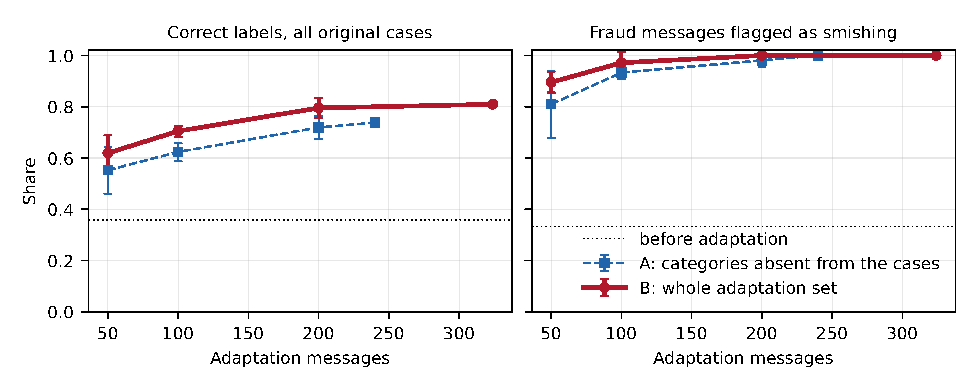
\includegraphics{figures/adaptation_curve}
\caption{Kazakhstan case study: adaptation of the character SVM with a synthetic set of Russian, Kazakh and English messages. Left: correct labels on the \val{kz-orig} original case-study messages; right: fraudulent messages labelled smishing. Points: mean $\pm$ standard deviation over five random subsets}
\label{fig:adaptation}
\end{figure*}

\emph{Adaptation.} We retrained the character SVM on the Mendeley training data together with a synthetic adaptation set of \val{kz-adapt-n} messages (\val{kz-adapt-ideas} message ideas in three languages, drafted with a language model and checked by the authors, with no near duplicates of the case-study messages). With the whole set (condition B), the fraudulent case-study messages labelled smishing rise from \val{kz-fraud-before} to \val{kz-fraud-after-b} of \val{kz-fraud-n}, and the share of correct labels from \val{kz-acc-before} to \val{kz-acc-after-b} (Fig.~\ref{fig:adaptation}). Using only message categories that do not occur in the case study (condition A) gives \val{kz-fraud-after-a} of \val{kz-fraud-n} and \val{kz-acc-after-a}. The macro F1 on the Mendeley validation data stays between \val{kz-val-min} and \val{kz-val-max}, against \val{kz-val-before} before adaptation, and the latency does not change. The price is false alarms. On the legitimate adaptation messages with links that were not used for training, the adapted models label between \val{kz-legit-link-min} and \val{kz-legit-link-max} correctly, about as many as before adaptation (\val{kz-legit-link-before}), but the errors move from spam to smishing: \val{kz-legit-link-smish-after}\% of these messages are flagged as smishing after adaptation against \val{kz-legit-link-smish-before}\% before. The genuine bank warning about a suspicious transaction is flagged as smishing by the adapted model in all three languages, and by all three models after translation. Because the adaptation set and the case-study messages were written in a similar style, these effects may be overestimated.

\emph{Real messages.} In public sources (news articles) we found only \val{kz-real-n} verbatim texts of fraudulent messages sent in Kazakhstan, one of them a fragment and one cut off in a screenshot. As written, the adapted character SVM labels \val{kz-real-flagged} of them smishing, with a confidence between \val{kz-real-conf-min} and \val{kz-real-conf-max}; the models without adaptation, the cascade and BERT label none of them smishing. After sentence-wise translation some of them are recognised by the other models, but \val{kz-real-never} message, a fragment that only reports a change in the status of a loan and contains no link or request, is labelled smishing by no model with either input. With so few messages this is an illustration only.

\subsection{Limitations}\label{sec:limitations}

\begin{itemize}
\item \emph{Small test classes.} The three-class test set has \val{men-test-smishing} smishing and \val{men-test-spam} spam messages, so one or two messages change the F1 score of these classes noticeably, and only large differences can be significant.
\item \emph{Significance on one seed.} The tests use the predictions of seed 1 and capture the variation of the test set, not that of training; for some conditions the spread between seeds is comparable to the differences between models.
\item \emph{Threshold.} $\tau^{*}$ was chosen on validation data with seeds \val{tau-seeds} and used for all seeds. In the binary settings the same criterion selected high thresholds (\val{tau-mh} in the Mahmud setting and up to \val{tau-tr-ft} for transfer), which send \val{routed-binary-min-pct}\% to \val{routed-binary-max-pct}\% of the messages to the transformer; there the cascade is close to the transformer in quality and much more expensive. Latency was measured only for the three-class task.
\item \emph{Selection on validation data.} Both stages were early-stopped on the clean validation data, and the hyperparameters of the baselines were tuned on it. This holds for all models, so the comparisons are fair, but validation scores were optimistic.
\item \emph{Obfuscation model.} The operations are simple and random; real senders choose their edits, may combine them with paraphrasing and may target the detector. The held-out family acts on Latin letters only, so on Cyrillic text it reduces mostly to letter doubling.
\item \emph{Re-implementation.} The published methods were re-implemented from their descriptions; settings that the papers do not state were chosen by us, and the data augmentation with generated messages of Shim et al. was not reproduced.
\item \emph{Cost.} $L_r$ uses the argmax rule and not a cost-sensitive threshold.
\item \emph{Duplicates.} The inflation analysis does not separate the effect of duplicates from that of conflicting labels.
\item \emph{Case study.} The Kazakhstan messages are few, written by the authors or synthetic, and the four real messages are not enough for any metric.
\end{itemize}
